% !Mode:: "TeX:UTF-8"
% !TEX program  = xelatex
% \section{\LaTeX\ 入门}
% 请参考 \href{https://tex.readthedocs.io/zh_CN/latest/}{在线文档},包括学习资源及学习路径。欢迎在 GitHub 上提出 \href{https://github.com/Iydon/tex/issues}{Issues}。
\section{实验}

\subsection{引言}
对于实验部分,首先本设计建立了与CAD模型相对应的仿真模型,然后在仿真模型上测试控制算法。而在进行实验之前,须进行相关的硬件准备,如系统集成和参数辨识,然后再将仿真中测试成功的控制算法转移到实物模型上。如前文所说,仿真器选用的是MATLAB Simulink,可以快速实现仿真到实物的迁移。而系统集成主要是侧重于将已经搭建好的电气系统使用状态机搭建抽象的通讯网络,以实现初始化和保证机器人在运行时的安全性。如前文建模控制部分所言,由于机器人所有可活动杆件都被视为质心以计算整体小车-倒立摆模型的转动惯量,因此参数辨识主要侧重与获取机器人重心,而非各杆件的转动惯量。

\subsection{仿真模型}
仿真选择MATLAB Simulink Simscapes,从而可以实现仿真与实物的快速迁移。此外,作为商业引擎,Simulink Simscapes提供了精准的仿真和接触力模型,从而获得更好的仿真效果。在本论文中,仿真模型对CAD模型和实物进行了一定程度的简化。考虑到前文机械设计的部分提到的平行四边形连杆机构,其活动的连杆相对于大腿的运动幅度不大,且该连杆的质量也较小,因此可以将之视为与大腿固连的连杆,从而在运动学上实现了远端驱动的等效,在动力学上实现了远端驱动的简化。

\begin{figure}[h!]
  \centering
  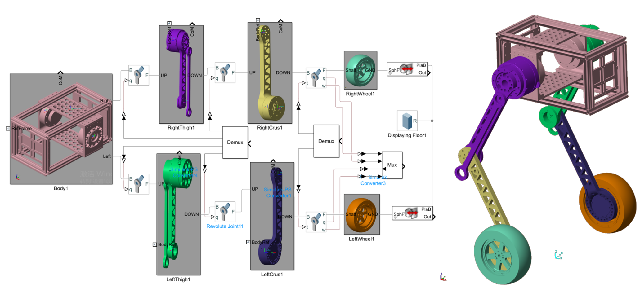
\includegraphics[width=1.0\linewidth]{figures/Sec5/simumod.png}
  \caption{
  左图:仿真模型搭建截图。右图:在Simulink可视化显示中的仿真3D模型。
  }
  \label{fig:sec5-simumod}
   \vspace{6pt}
\end{figure}


对于具体在仿真系统搭建模型,首先在CAD中导出每个零部件的通用3D文件(如STEP文件),然后分别导入仿真器,再每个零部件上根据实际情况定义坐标系,然后在坐标系之间定义位姿变换和运动副。这些零件和它们的坐标系被封装在一个子系统中,并且被增加了坐标系和零件的截图做的蒙版以方便区分,其与在MATLAB Simulink中仿真可视化界面展示的结果如图\ref{fig:sec5-simumod}所示,而其封装后,与控制器等如图\ref{fig:sec5-simuabs}所示。值得注意的是,上述部件使用转动副连接是针对机器人本身,而机器人与地面的交互则通过接触力模型来实现。根据理想机器人假设,机器人与地面的接触被认为是球-面接触,且机器人仅能沿轮子前后反向运动,而不能沿左右方向运动,满足非完整约束方程。但需要开始仿真,则需要定义机器人与世界系之间的虚拟6自由度关节,并给定初始条件。


\begin{figure}
  \centering
  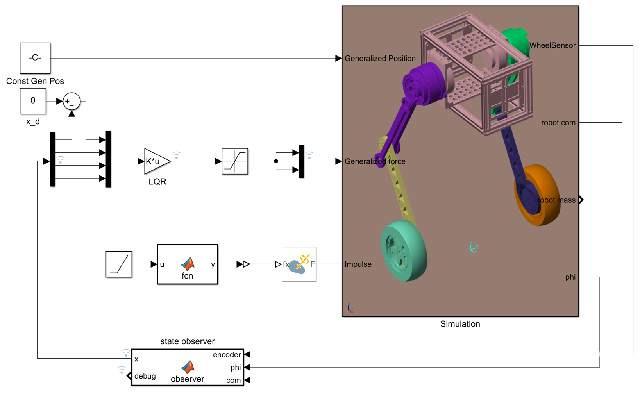
\includegraphics[width=0.85\linewidth]{figures/Sec5/simuabs.png}
  \caption{
  仿真封装示意图,其中右半部分被封装起来的部分是仿真器本身,接受位置和力指令,反馈机器人的状态。在本图中,使用了一个LQR控制器以同时实现平衡和轨迹跟踪。
  }
  \label{fig:sec5-simuabs}
   \vspace{6pt}
\end{figure}

\subsection{仿真实验}
在仿真实验中,主要实验目的是测试静态平衡,具体包括初始从一个非平衡的角度恢复至平衡状态,和受到外力扰动下重新回复到稳定状态的实现。在此基础上,测试矢状面的轨迹跟踪,具体为给定目标位置,机器人前往目标位置。如图\ref{fig:sec5-simuabs}所示,这里展示的是使用LQR控制器实现上述轨迹跟踪。使用针对轮子编码器进行加权和饱和的PID控制可以达到类似的效果。考虑到封装了仿真模型,因此上述控制器的切换较为简单。实际上仿真也实现了矢状面的轨迹跟踪,通过Simulink自带的滑块组件改变需要跟踪的位置值,即可实现机器人的轨迹跟踪。考虑到论文难以展示视频,因此主要集中在展示倾角恢复和抗扰两个方面。首先是倾角恢复,如图\ref{fig:sec5-lqr1}所示,机器人初始的质心与重锤线有0.1弧度(约6角度)的偏差,然后机器人在3秒的时间恢复平衡,并同时回到了原点的位置。而受到外界扰动恢复的实验中,如图\ref{fig:sec5-lqr2}所示,机器人首先在平衡状态下,当仿真时间在2s时,机器人受到大小为2Ns的冲量,随后在仿真时间5s时恢复平衡,且也恢复到原先的平衡点。仿真实验表明,使用先前章节所介绍的LQR控制器,起到了较好的平衡效果。可以看到当受到外力扰动时,机器人瞬间获得了角速度,然后通过加速移动改变质心位置,从而使用重力矩产生的冲量抵消外力产生的冲量。然后机器人的LQR控制器寻找到恢复到原先所在平衡点的路线,从而在角度和位移上恢复了原先的状态。

\begin{figure}
  \centering
  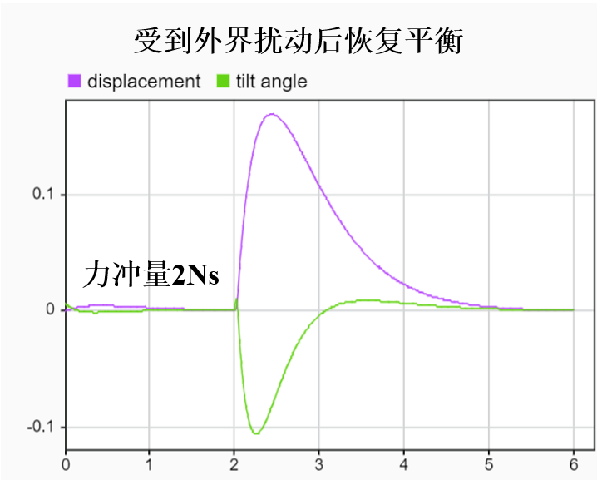
\includegraphics[width=0.6\linewidth]{figures/Sec5/lqr1.png}
  \caption{
  倾角恢复实验。机器人初始的质心与重锤线有0.1弧度(约6角度)的偏差,然后机器人在3秒的时间恢复平衡,并同时回到了原点的位置。
  }
  \label{fig:sec5-lqr1}
   \vspace{6pt}
\end{figure}

\begin{figure}[h]
  \centering
  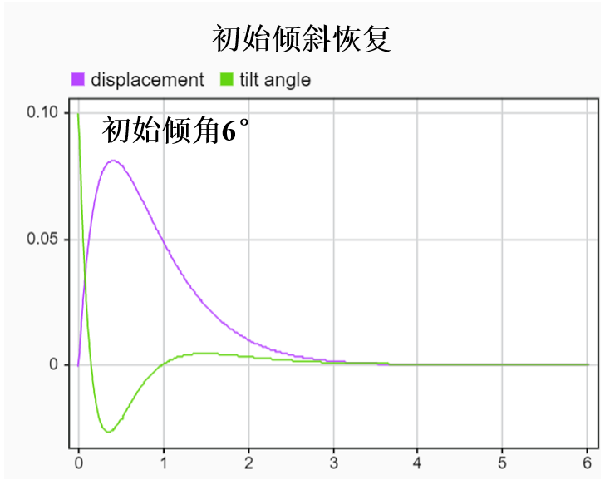
\includegraphics[width=0.6\linewidth]{figures/Sec5/lqr2.png}
  \caption{
  受到外界扰动恢复实验。机器人首先在平衡状态下,当仿真时间在2s时,机器人受到大小为2Ns的冲量,随后在仿真时间5s时恢复平衡,且也恢复到原先的平衡点。
  }
  \label{fig:sec5-lqr2}
   \vspace{6pt}
\end{figure}

\subsection{硬件准备}
如第二章所述,电气系统和控制系统的硬件上拥有2组不同的抽象控制网络,并且需要内置位置限制、电机使能和静能逻辑、电流限制和软件急停,因此需在再SpeedGoat内设计控制状态机,作为机器人控制器的底层保障系统。第二层系统反馈数据网络已由Simulink EtherCAT包封装好。另外如第四章所述,实物需要重新测定质心,因此采用了悬线测量法,通过IMU读取悬空静止角度得出重力方向,从而通过不同铅垂线交点获得质心位置。

\subsubsection{系统集成}
状态机主要包括以下几种状态。初始化进入状态,此时电机等待使能命令。使能状态,如前文所述,电机使能需要多次读取控制器STATUS WORD并发送CMD WORD,因此在获得遥控器的使能指令之后,所有电机会并行执行上述使能指令,并且根据驱动器反馈使能是否成功决定重新使能或进入下一个状态。下一个状态是等待新的位置指令状态,考虑到膝盖和胯部电机均工作在位置模式下,因此在使能之后,只有移动位置控制器才会激活膝盖电机和胯部电机的移动,以防止使能状态与位置滑块停留所代表的位置相差过大,误发送位置指令的情况。获得了新的位置指令之后,电机会进入执行位置指令的模式,并直到执行完之后,不接受新的位置指令。考虑到驱动器内建的位置模式刚性较大,因此实际上位置模式的实现是通过微小的位移量叠加而成。在将来的工作中,也可以设计成使用梯形曲线进行运动规划,从而可以在运动的过程中途改变目标位置。值得注意的是,轮子电机工作在扭矩或速度模式下,取决了控制器是LQR还是PID。但实际上在上述的四个状态中,在所有电机完成使能之后,平衡控制器就会自动开启,从而实现平衡和轨迹跟踪的功能。状态机的设计如图\ref{fig:sec5-stateflow}所示。值得注意的是,在任意状态下,接收到静能或软件急停指令时,状态机都会跳转到等待使能的状态并关闭迪纳基输出。而在位置跟踪的过程中,状态机会保证位置不会超过机械限位,同时会监看电流大小。当电流过大时,会退出位置跟踪状态并进入等待位置跟踪状态,以停止电流继续增大。

\begin{figure}
  \centering
  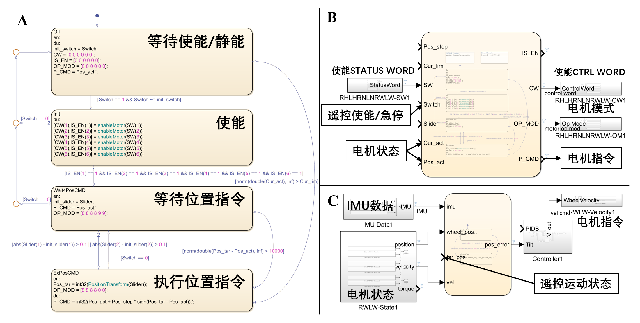
\includegraphics[width=1.0\linewidth]{figures/Sec5/stateflow.png}
  \caption{
  状态机示意图。其中左边的是状态机的四种状态。右边展示了状态机封装后的效果,左右分别是其输入和输出变量,用于和Simulink的其他模块交互。
  }
  \label{fig:sec5-stateflow}
   \vspace{6pt}
\end{figure}

\subsubsection{参数辨识}

\begin{figure}[h!]
  \centering
  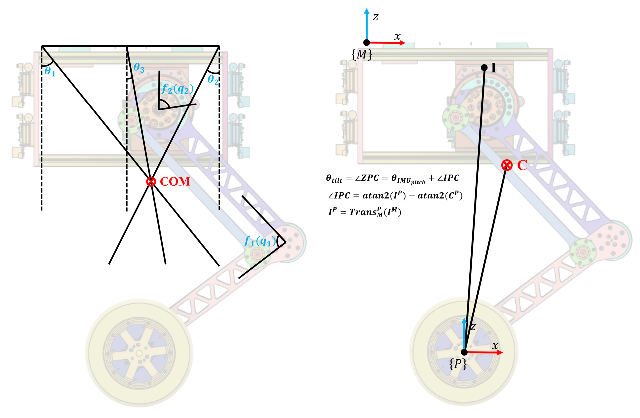
\includegraphics[width=0.85\linewidth]{figures/Sec5/comdata.png}
  \caption{
  质心测量示意图。根据这些几何关系,可以求出特定坐标系下的质心位置,从而通过最小二乘计算每个杆件在矢状面的质心位置。
  }
  \label{fig:sec5-comdata}
   \vspace{6pt}
\end{figure}

考虑到CAD模型与实际机器人在质心分布上有较大差异,如电机质量分布、轴承、螺丝、电线未计算在内,因此需要测定每个杆件的质心。传统上质心的测量方法是线悬法,但这里因为需要测量三维空间的质心,难度较大,且电线、轴承、螺丝等拆卸则无测定意义,因此会将整个机器人视作一个整体测定,而通过多组数据最小二乘计算出每个杆件的质心。考虑到目前机器人左右腿变高度是同步的,因此仅需要测定每个杆件在矢状面中的质心。如前文所述,根据机器人的运动学,假设每个杆件的质心位置为某变量后,可以计算出带变量的整体质心位置。

拥有多组数据后,便可以通过求解过约束线性方程组(最小二乘)实现质心的计算。虽然机器人质心可以通过在相同的构型下进行多次悬挂,同样针对质心位置计算另一次最小二乘,但实际上通过多组实验也可以实现减少误差的效果,因此在机器人已知位置设置两个悬挂点,然后在每个悬挂点悬挂时,改变机器人的构型,通过IMU记录重力方向,对第二个悬挂点也采用相同的方式。在采集了机器人构型数据和对应的IMU数据之后,在相同构型下, 通过重力方向可以计算出质心位置,计算方式如图\ref{fig:sec5-comdata}所示。值得注意的是,考虑到左右腿的同步性,其质量应当计算为原本2倍以得到正确的质心位置结果。


\subsection{实物实验}

\begin{figure}[h!]
  \centering
  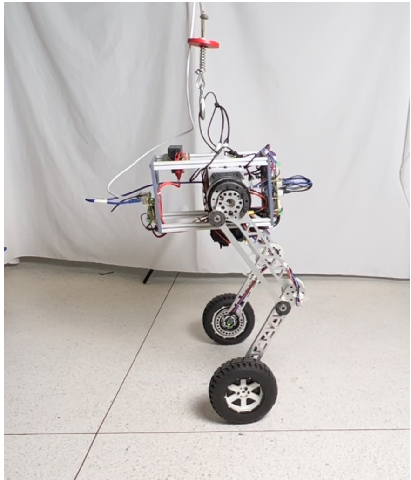
\includegraphics[width=0.45\linewidth]{figures/Sec5/simplerealresult.png}
  \caption{
  基于PID的实物静态平衡实验结果。可以看到其安全绳处于松弛状态,依靠平衡控制器实现了平衡。
  }
  \label{fig:sec5-simplerealresult}
   \vspace{6pt}
\end{figure}

基于上述内容,实物实验主要是将仿真实验转移到实物上。对于仿真模型,其质心位置根据仿真器的配置文件,通过机器人构型计算出,而实物则由测定的数据和机器人构型计算出,因此对于控制器而言,这个数据是“隐形”的,因为控制器仅需指导质心位置与竖直线间夹角即可。实物实验同样包括静态平衡和轨迹跟踪,在目前采用叠加位置跟踪的PID控制器与开环差速转向的情况下,其中平衡的效果如图\ref{fig:sec5-simplerealresult}所示,可以看到其安全绳出于松弛状态,依靠平衡控制器实现了平衡。此外,图\ref{fig:sec5-static}展示了其在延时摄影下的的平衡状态,可见机器人会以极慢的速度在极小范围内振荡,考虑到机器人实物原型机与控制模型的若干误差,可以认为机器人实际上已经达到平衡状态。

\begin{figure}[h!]
  \centering
  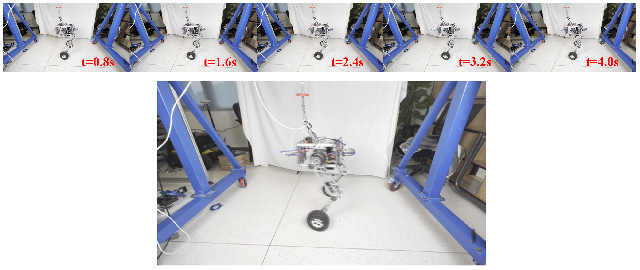
\includegraphics[width=1.0\linewidth]{figures/Sec5/static.png}
  \caption{
  基于PID的实物静态平衡实验结果。上图是平衡视频关键帧截图,下图是将关键帧叠加展示。
  }
  \label{fig:sec5-static}
   \vspace{6pt}
\end{figure}

\begin{figure}[h!]
  \centering
  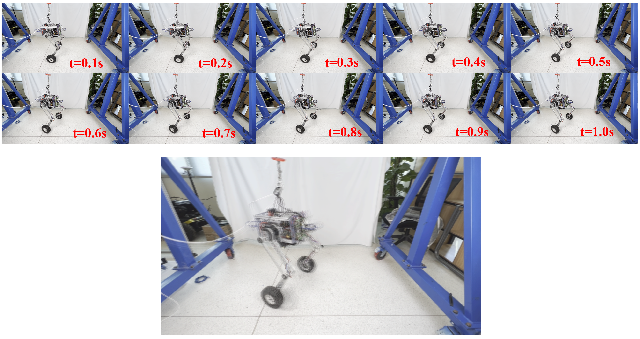
\includegraphics[width=1.0\linewidth]{figures/Sec5/rot.png}
  \caption{
  基于叠加位置跟踪的PID控制器与开环差速转向的实物原地自转的实验结果。上图是视频关键帧截图,下图是将关键帧叠加展示。
  }
  \label{fig:sec5-rot}
   \vspace{6pt}
\end{figure}

同样的,该控制器也实现了机器人在空间中的轨迹跟踪。为方便具体实现,给定轨迹为机器人质心处的定高度轨迹。据此,可以计算出每时刻机器人的质心速度,而考虑到机器人驱动轮为2自由度,因此需要根据若干时间窗口内的速度计算出机器人整体(此时机器人视为单一刚体)的角速度,则根据移动机器人的运动学方程(公式\ref{eq:naveq}),可以用于产生相应角速度的每轮线速度差速。这里不采用移动机器人运动学方程直接计算出每个轮子的速度,是考虑到欠驱动机器人,尤其是本轮腿机器人,最优先考虑的是平衡,因此具体的质心线速度和机器人角速度的实现分别需要融合在平衡控制器中,而不能单独实现。如图\ref{fig:sec4-3dsimple}和图\ref{fig:sec4-3dpid}所示的控制器可以实现线速度和角速度的闭环和开环控制。值得注意的是,机器人的线速度追踪采用对机器人在矢状面上位置点跟踪的方式实现,因此在输入控制器之前需要进行积分,这样设计的目的是使机器人不至于维持一个恒定的加速度平衡,或在受到外力扰动后可以获得一个返回原位置的趋势。而差速转向是开环控制,因此实际上机器人在实现轨迹跟踪时,仍需要一个更高层的控制器实现轨迹跟踪的反馈。考虑到机器人在非结构化的环境中活动且可能随时受到外界扰动,因此参考文献\cite{klemm2019ascento}中所述,将这个更高层的控制器认为是路径规划中的一部分,相应的本轮腿机器人则可以接受实时的、片段的轨迹,而不需要事先接受所有轨迹。


\begin{figure}[h]
  \centering
  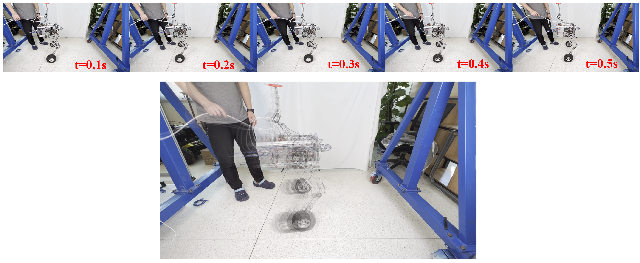
\includegraphics[width=1.0\linewidth]{figures/Sec5/movfd.png}
  \caption{
  基于叠加位置跟踪的PID控制器与开环差速转向的实物直线前进的实验结果。上图是视频关键帧截图,下图是将关键帧叠加展示。
  }
  \label{fig:sec5-movfd}
   \vspace{6pt}
\end{figure}


实际实验中,考虑安全性,机器人被安全绳限制在一定的活动范围内,且如上文所论述,实验主要测试机器人实现定速自转与定速直线运动。图\ref{fig:sec5-rot}是定速自转的截图,分别包括视频关键帧截图(每间隔0.1s为1关键帧),与关键帧叠加展示。考虑到实验条件,机器人自转速度较慢,但可通过第一张与最后一张关键帧明显看出机器人转动了约$\frac{\pi}{4} rad$,证明该控制器可以在保持平衡的状态下实现定速自转。

图\ref{fig:sec5-movfd}是则展示了定速直线运动的截图,也分别包括视频关键帧截图(每间隔0.1s为1关键帧),与关键帧叠加展示。通过关键帧的叠加显示可以明显看出机器人实现了定速直线运动,证明该控制器可以在保持平衡的状态下实现定速直线运动。

\subsection{本章小结}

在本章中,首先介绍了用于验证算法的仿真模型的搭建,以及之前章节中提到的算法在仿真模型上的验证。然后介绍了为原型机实验所做的准备,包括机器人的参数辨识与机电系统的集成。最后介绍了实物实验的具体设置、控制器,并分析了实验结果。